\documentclass[10pt]{article}
\usepackage[margin=0.78in]{geometry}
\usepackage{booktabs}
\usepackage{graphicx}
\usepackage{microtype}
\usepackage{xcolor}
\usepackage[hidelinks,hypertexnames=false]{hyperref}
\usepackage{float}
\usepackage{placeins}
\usepackage{amsmath}

\newcommand{\protocol}{team-formation protocol}
\hypersetup{
  pdftitle={Absolute Multi-Agent Performance Across Scale},
  pdfauthor={AlemDICE scaling study},
  pdfsubject={Descriptive scaling analysis from one to thirty-two agents}
}

\title{\textbf{Absolute Multi-Agent Performance Across Scale}\\
\large Descriptive analysis from one to thirty-two agents}
\author{AlemDICE scaling study}
\date{July 2026}

\begin{document}
\maketitle

\begin{abstract}
This report analyzes absolute, rather than population-normalized, performance
over two completed scaling campaigns.  An earlier baseline screen contains
three seeds at \(N\in\{1,2,3,4,6\}\), while a matched comparison contains one
200-step episode for baseline and \protocol{} at
\(N\in\{8,16,32\}\).  The principal result is a positive protocol return
advantage at every matched scale, accompanied by a larger share of coordinated
achievement unlocks.  The advantage is not uniform: acceleration is strongest
from 8 to 16 agents and weakens from 16 to 32, exposing a concrete
diminishing-yield regime.  Because the matched cells contain only one seed,
these are effect-size observations and mechanism diagnostics, not estimates of
statistical significance.
\end{abstract}

\section{Design and estimands}

The two campaigns are deliberately analyzed separately.  The earlier screen
uses seeds 13100--13102 and reports means, observed ranges, and sample
coefficients of variation.  The matched campaign uses seed 14100 in every
condition and reports paired descriptive contrasts.  A dotted break in the
all-scale figure marks the campaign boundary; no line is drawn between the
six- and eight-agent baseline cells.

The main absolute estimands are
\[
R_{\mathrm{team}} = N\,\bar R_{\mathrm{agent}},
\qquad
A_{\mathrm{sum}} = \sum_{i=1}^{N}\sum_k
\mathbf{1}\{\text{agent }i\text{ first-unlocked achievement }k\}.
\]
Thus \(R_{\mathrm{team}}\) is the return summed over physical agents, and
\(A_{\mathrm{sum}}\) counts an achievement once for each agent that first
unlocks it.  Team-unique achievement types are reported separately and count
each type at most once.  These quantities answer whether adding agents produces
more total work; they do not divide away population size.

\begin{figure}[H]
\centering
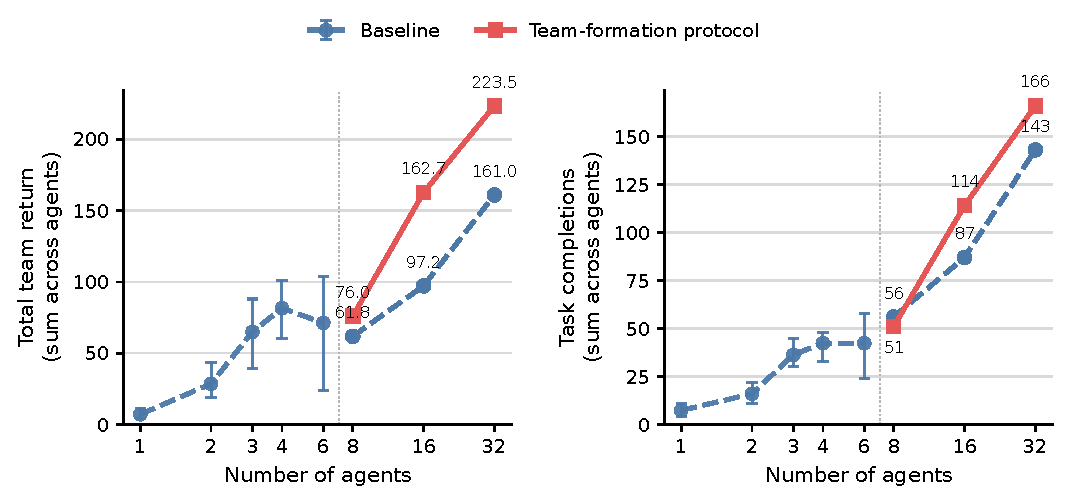
\includegraphics[width=\linewidth]{../../Figures/20260721_absolute_team_performance_all_scales.pdf}
\caption{Absolute team output across the two campaigns.  Task completions count
only the first completion of each task by each agent.  Whiskers at
\(N\leq6\) are observed three-seed ranges.  Points at \(N\geq8\) are single
matched episodes.  The vertical dotted line denotes the campaign boundary.}
\label{fig:absolute-all}
\end{figure}

\section{Earlier baseline screen: a capacity knee}

\begin{table}[t]
\centering
\small
\setlength{\tabcolsep}{4.5pt}
\begin{tabular}{rrrrrr}
\toprule
$N$ & Team return & Return/agent & Agent unlocks & Unique types & Return CV \\
\midrule
1 & 7.1 [4.0, 11.0] & 7.13 & 7.3 [4, 11] & 7.3 & 49.9\% \\
2 & 28.6 [19.0, 43.7] & 14.28 & 16.0 [11, 22] & 10.3 & 46.4\% \\
3 & 65.0 [39.3, 88.0] & 21.68 & 36.3 [30, 45] & 19.3 & 37.6\% \\
4 & 81.5 [60.2, 101.2] & 20.37 & 42.3 [33, 48] & 19.3 & 25.2\% \\
6 & 71.3 [23.8, 103.6] & 11.88 & 42.3 [24, 58] & 15.0 & 58.9\% \\
\bottomrule
\end{tabular}
\caption{Earlier baseline screen. Team return and agent unlocks are means with observed three-seed ranges in brackets. CV is the sample coefficient of variation of absolute team return. Each cell requested 200 steps; one three-agent episode terminated naturally at step 191.}
\label{tab:low-scale}
\end{table}


Absolute baseline return rises sharply from 7.1 at one agent to 81.5 at four
agents, an \(11.4\times\) increase for a \(4\times\) population increase.
Summed achievement unlocks increase \(5.8\times\), from 7.3 to 42.3.  This
superlinear early region is consistent with task parallelism and access to
multi-agent opportunities, but it is not a clean causal estimate: population
also changes spawn geometry, pressure, specialization balance, and available
coordination.

The screen then exhibits a knee.  Moving from four to six agents reduces mean
absolute return by 12.5\% (81.5 to 71.3), leaves mean summed unlocks exactly
flat at 42.3, and reduces unique team achievement types from 19.3 to 15.0.
The six-agent return CV is 58.9\%, the largest in the screen, compared with
25.2\% at four agents.  This is evidence of unstable saturation in the
baseline-as-implemented, not evidence that six agents are intrinsically worse:
the original campaign documents a geometric-feasibility confound at \(N=6\).

\section{Matched protocol comparison}

\begin{table}[t]
\centering
\small
\setlength{\tabcolsep}{4pt}
\begin{tabular}{rrrrrrrr}
\toprule
$N$ & Return B & Return P & $\Delta$ return & Unlocks B & Unlocks P & $\Delta$ unlocks & Unique B/P \\
\midrule
8 & 61.8 & 76.0 & +23.0\% & 56 & 51 & -8.9\% & 14/19 \\
16 & 97.2 & 162.7 & +67.4\% & 87 & 114 & +31.0\% & 15/16 \\
32 & 161.0 & 223.5 & +38.8\% & 143 & 166 & +16.1\% & 18/21 \\
\bottomrule
\end{tabular}
\caption{Matched absolute performance. B denotes baseline and P denotes the team-formation protocol. Each value is one 200-step episode at the same seed; deltas are descriptive, not confidence intervals.}
\label{tab:matched-absolute}
\end{table}


\begin{figure}[H]
\centering
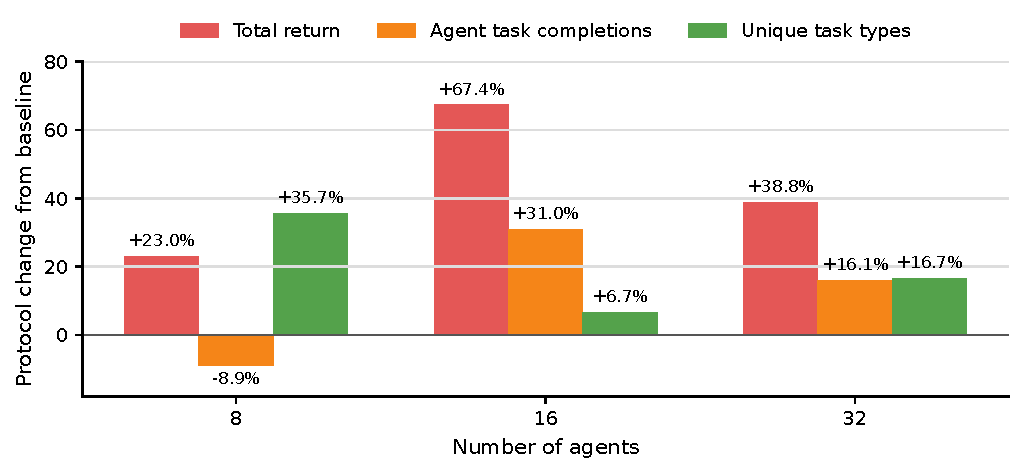
\includegraphics[width=0.94\linewidth]{figures/protocol_uplift.pdf}
\caption{Protocol change relative to the matched baseline.  Task completions
count only the first completion of each task by each agent.  Return improves at
all three scales.  The eight-agent cell combines higher return and broader
team-unique coverage with fewer summed per-agent task completions, revealing a
quality/breadth versus repetition tradeoff.}
\label{fig:uplift}
\end{figure}

\subsection{Finding 1: positive return signal at every matched scale}

The protocol increases absolute return by 23.0\% at eight agents, 67.4\% at
16 agents, and 38.8\% at 32 agents.  In raw units the gains are 14.2, 65.5,
and 62.5.  The 32-agent result is therefore not merely an artifact of a
percentage denominator: it retains nearly the full 16-agent absolute gain.
Nevertheless, one seed cannot establish robustness or a population-level
confidence interval.

\subsection{Finding 2: the eight-agent result favors breadth over repetition}

At eight agents the protocol produces 51 summed unlocks versus 56 for baseline
(\(-8.9\%\)), yet reaches 19 unique team achievement types versus 14
(\(+35.7\%\)) and earns 23.0\% more return.  The protocol therefore did not
win by having every agent repeat more easy milestones.  It covered more
distinct achievement types and shifted activity toward coordinated events.
This is a useful mechanism signal: raw unlock volume alone would incorrectly
classify the eight-agent result as worse.

\section{Coordination composition}

\begin{table}[t]
\centering
\small
\setlength{\tabcolsep}{5pt}
\begin{tabular}{rrrrrrrr}
\toprule
$N$ & Base B & Coord B & Share B & Base P & Coord P & Share P & Coord count ratio \\
\midrule
8 & 54 & 2 & 3.6\% & 43 & 8 & 15.7\% & 4.00$\times$ \\
16 & 83 & 4 & 4.6\% & 103 & 11 & 9.6\% & 2.75$\times$ \\
32 & 138 & 5 & 3.5\% & 149 & 17 & 10.2\% & 3.40$\times$ \\
\bottomrule
\end{tabular}
\caption{Composition of summed agent first-unlocks. ``Base'' denotes individual-task achievements and ``Coord'' coordinated achievements.}
\label{tab:composition}
\end{table}


\begin{figure}[H]
\centering
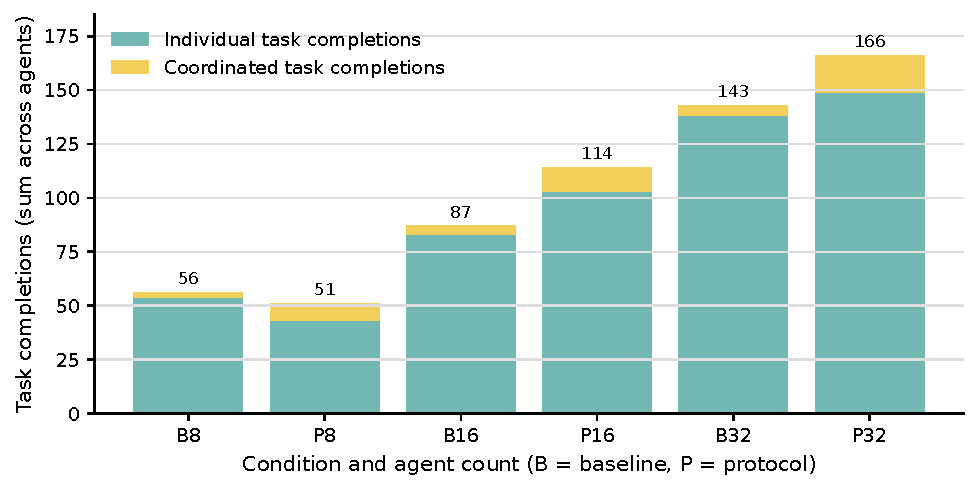
\includegraphics[width=0.90\linewidth]{figures/achievement_composition.pdf}
\caption{Individual and coordinated first task completions summed across
agents.  Each adjacent pair compares baseline (B) and protocol (P) at the
same population.}
\label{fig:composition}
\end{figure}

\subsection{Finding 3: coordinated achievements are the most consistent
mechanism signal}

The coordinated-unlock count rises from 2 to 8 at \(N=8\), from 4 to 11 at
\(N=16\), and from 5 to 17 at \(N=32\): multipliers of \(4.00\times\),
\(2.75\times\), and \(3.40\times\).  Coordinated unlocks constitute only
3.5--4.6\% of baseline unlocks, but 9.6--15.7\% under the protocol.  Unlike
total unlock volume, this directional signal is positive at every matched
scale and directly reflects the intended behavioral mechanism.

The effect is not only substitution.  At 16 and 32 agents, individual-task
unlocks also increase (83 to 103 and 138 to 149), while coordinated unlocks
increase more sharply.  At eight agents individual-task unlocks fall from 54
to 43, making that cell the clearest example of specialization reducing
redundant individual progress while expanding team-level breadth.

\section{Scaling efficiency and diminishing marginal yield}

\begin{figure}[H]
\centering
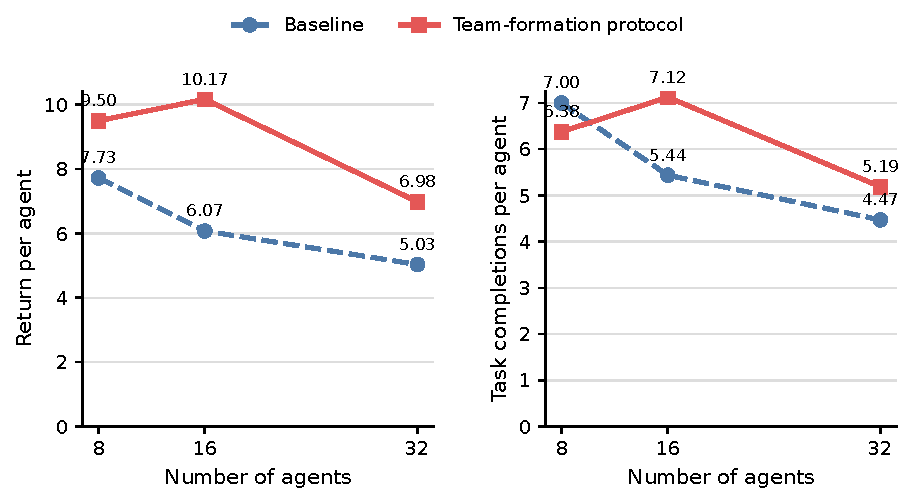
\includegraphics[width=\linewidth]{figures/per_agent_efficiency.pdf}
\caption{Per-agent efficiency in the matched campaign.  These normalized
diagnostics explain the absolute curves; they are not the primary performance
estimands.}
\label{fig:efficiency}
\end{figure}

\begin{table}[t]
\centering
\small
\setlength{\tabcolsep}{5pt}
\begin{tabular}{llrrrr}
\toprule
Condition & Interval & $\alpha_R$ & $\alpha_A$ & Marginal return & Marginal unlocks \\
\midrule
Baseline & 8$\rightarrow$16 & 0.653 & 0.636 & 4.42 & 3.88 \\
Baseline & 16$\rightarrow$32 & 0.728 & 0.717 & 3.99 & 3.50 \\
Protocol & 8$\rightarrow$16 & 1.098 & 1.160 & 10.84 & 7.88 \\
Protocol & 16$\rightarrow$32 & 0.458 & 0.542 & 3.80 & 3.25 \\
\bottomrule
\end{tabular}
\caption{Local scaling diagnostics. Elasticity $\alpha=\log(Y_1/Y_0)/\log(N_1/N_0)$; $\alpha=1$ is linear absolute scaling. Marginal columns report added output per added agent.}
\label{tab:scaling-diagnostics}
\end{table}


For output \(Y\), define the local scaling elasticity
\(\alpha=\log(Y_1/Y_0)/\log(N_1/N_0)\).  Linear absolute scaling has
\(\alpha=1\), sublinear scaling has \(\alpha<1\), and superlinear scaling has
\(\alpha>1\).

\subsection{Finding 4: the protocol's strongest scaling phase is 8 to 16}

From 8 to 16 agents, protocol return has elasticity 1.098 and unlock volume
has elasticity 1.160, both slightly superlinear.  Baseline elasticities are
0.653 and 0.636.  Each added agent in this interval yields 10.84 additional
return units and 7.88 additional unlocks under the protocol, versus 4.43 and
3.88 for baseline.

From 16 to 32 agents, protocol elasticities fall to 0.458 for return and 0.542
for unlocks.  The protocol remains absolutely better, but its marginal yield
falls to 3.80 return units and 3.25 unlocks per added agent, close to baseline's
3.99 and 3.50.  This pattern localizes the next research problem: beyond 16
agents, additional team structure preserves an output lead but no longer
creates superior marginal scaling.

\begin{figure}[H]
\centering
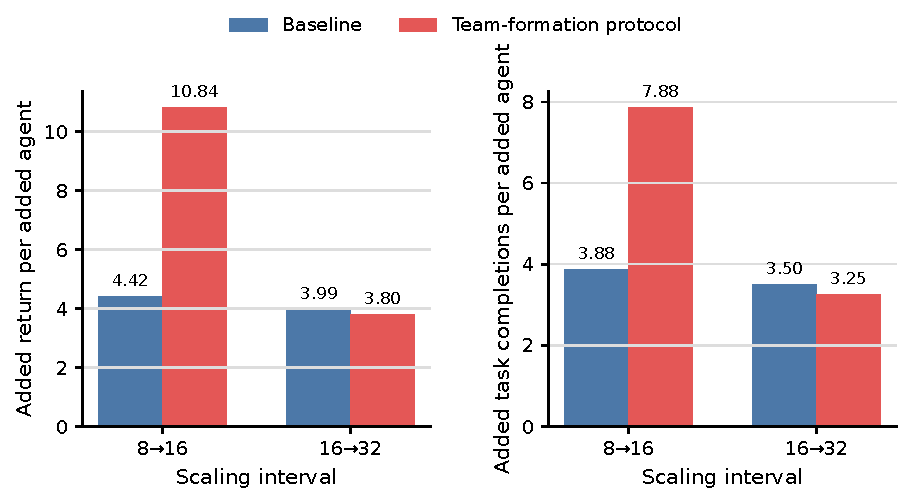
\includegraphics[width=\linewidth]{figures/marginal_yield.pdf}
\caption{Marginal absolute output per added physical agent.  Task completions
count only the first completion of each task by each agent.  The protocol's
large advantage in the 8-to-16 transition nearly disappears in the
16-to-32 transition.}
\label{fig:marginal}
\end{figure}

\subsection{Finding 5: the protocol mitigates, but does not eliminate,
per-agent decay}

Across 8 to 32 agents, baseline return per agent falls from 7.73 to 5.03
(\(-34.9\%\)); protocol return per agent falls from 9.50 to 6.98
(\(-26.5\%\)).  Summed unlocks per agent fall from 7.00 to 4.47 for baseline
and from 6.38 to 5.19 for the protocol.  The protocol therefore retains more
useful output per agent at the largest scale, especially in achievements, but
does not achieve scale-invariant efficiency.

\section{Interpretation and next experiments}

The data support three bounded claims.  First, the protocol has a positive
absolute-return signal at all matched scales.  Second, it consistently
increases coordinated achievement activity and team-level breadth.  Third,
the scaling mechanism changes regime: strong gains through 16 agents give way
to diminishing marginal yield by 32 agents.

The following experiments are the shortest path from signal to evidence:
\begin{enumerate}
  \item Repeat every \(N\in\{8,16,32\}\) matched cell for at least three,
  preferably ten, common seeds.  Report paired seed differences and bootstrap
  intervals rather than intervals over unmatched episodes.
  \item Instrument formation overhead: messages, delivered bytes, inactive
  turns, reassignment counts, and time-to-first coordinated unlock.  This can
  distinguish communication saturation from environmental saturation.
  \item At 32 agents, compare one global team with two and four independent
  teams while holding the physical population and task cap fixed.  The current
  marginal-yield collapse predicts that partitioning should restore local
  planning efficiency.
  \item Preserve the achievement decomposition.  Primary outcomes should
  include return, summed unlocks, unique types, and coordinated unlocks; any
  one of these alone misses the eight-agent tradeoff.
\end{enumerate}

\section{Limitations}

The high-scale comparison has one seed per cell, so no claim here is a
statistical significance claim.  The low- and high-scale campaigns use
different seeds and experimental configurations; their points are juxtaposed
to show coverage, not treated as one matched response curve.  Achievement
first-unlocks are cumulative binary events, not counts of repeated task
completion.  Finally, absolute output naturally tends to rise with population;
the efficiency and marginal-yield diagnostics are required to determine
whether those gains are proportional to the additional agents.

\end{document}
